\section{Durchführung}
\label{sec:Durchführung}
\begin{figure}[H]
  \centering
  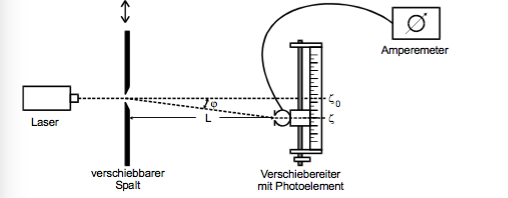
\includegraphics[height=7cm]{Aufbau.png}
  \caption{Versuchsaufbau \cite{skript}.}
  \label{fig:aufbau}
\end{figure}
Wie in Abbildung \ref{fig:aufbau} zu sehen ist, wird bei diesem Versuch ein
verschiebbarer Einzel- oder Doppelspalt von einem Laser mit einer Wellenlänge von
etwa $\SI{650}{\nano\meter} $ beleuchtet, sodass sich dahinter ein Beugungsbild
ausbildet. Dieses wird von einem lichtempfindlichen Detektor auf einem
Verschiebereiter mittels einer Photodiode ausgemessen.
Es ist dabei darauf zu achten, dass der der Detektor einen
möglichst großen Abstand zum Spalt, also mindestens einen Meter, besitzt.
Zudem muss vor Versuchsbeginn auch der Dunkelstrom gemessen werden, welcher
von den Messwerten jeweils abgezogen wird.
Es wird nun bei konstanten Lichtverhältnissen je eine Messreihe zu einem Einzelspalt
und zu zwei verschiedenen Doppelspalten aufgenommen, wobei je mindestens 50
Messwerte genommen werden und das Hauptmaximum sowie beim Einzelspalt mindestens ein
und bei den Doppelspalten mindestens zwei Nebenmaxima auf beiden Seiten gemessen werden
